\documentclass[11pt]{article}

%% MinionPro fonts 
%\usepackage[lf]{MinionPro}
%\usepackage{MnSymbol}
\usepackage{microtype}

%% Margins
\usepackage{geometry}
\geometry{verbose,letterpaper,tmargin=1in,bmargin=1in,lmargin=1in,rmargin=1in}

%% Other packages
\usepackage{amsmath}
\usepackage{amsthm}
\usepackage[shortlabels]{enumitem}
\usepackage{titlesec}
\usepackage{soul}
\usepackage{tikz}
\usepackage{mathtools}
\usepackage{pgfplots}
\usepackage{tikz-3dplot}
\usepackage{algorithmic}
\usepackage[export]{adjustbox}
\usepackage{tcolorbox}
\usepackage{optprog}

%% Paragraph style settings
\setlength{\parskip}{\medskipamount}
\setlength{\parindent}{0pt}

%% Change itemize bullets
\renewcommand{\labelitemi}{$\bullet$}
\renewcommand{\labelitemii}{$\circ$}
\renewcommand{\labelitemiii}{$\diamond$}
\renewcommand{\labelitemiv}{$\cdot$}

%% Colors
\definecolor{rred}{RGB}{204,0,0}
\definecolor{ggreen}{RGB}{0,145,0}
\definecolor{yyellow}{RGB}{255,185,0}
\definecolor{bblue}{rgb}{0.2,0.2,0.7}
\definecolor{ggray}{RGB}{190,190,190}
\definecolor{ppurple}{RGB}{160,32,240}
\definecolor{oorange}{RGB}{255,165,0}

%% Shrink section fonts
\titleformat*{\section}{\normalsize\bf}
\titleformat*{\subsection}{\normalsize\bf}
\titleformat*{\subsubsection}{\normalsize\it}

% %% Compress the spacing around section titles
\titlespacing*{\section}{0pt}{1.5ex}{0.75ex}
\titlespacing*{\subsection}{0pt}{1ex}{0.5ex}
\titlespacing*{\subsubsection}{0pt}{1ex}{0.5ex}

%% amsthm settings
\theoremstyle{definition}
\newtheorem{problem}{Problem}
\newtheorem{example}{Example}
\newtheorem*{theorem}{Theorem}
\newtheorem*{bigthm}{Big Theorem}
\newtheorem*{biggerthm}{Bigger Theorem}
\newtheorem*{bigcor1}{Big Corollary 1}
\newtheorem*{bigcor2}{Big Corollary 2}

%% tikz settings
\usetikzlibrary{calc}
\usetikzlibrary{patterns}
\usetikzlibrary{decorations}
\usepgfplotslibrary{polar}

%% algorithmic setup
\algsetup{linenodelimiter=}
\renewcommand{\algorithmiccomment}[1]{\quad// #1}
\renewcommand{\algorithmicrequire}{\emph{Input:}}
\renewcommand{\algorithmicensure}{\emph{Output:}}

%% Answer box macros
%% \answerbox{alignment}{width}{height}
\newcommand{\answerbox}[3]{%
  \fbox{%
    \begin{minipage}[#1]{#2}
      \hfill\vspace{#3}
    \end{minipage}
  }
}

%% \answerboxfull{alignment}{height}
\newcommand{\answerboxfull}[2]{%
  \answerbox{#1}{6.38in}{#2} 
}

%% \answerboxone{alignment}{height} -- for first-level bullet
\newcommand{\answerboxone}[2]{%
  \answerbox{#1}{6.0in}{#2} 
}

%% \answerboxtwo{alignment}{height} -- for second-level bullet
\newcommand{\answerboxtwo}[2]{%
  \answerbox{#1}{5.8in}{#2}
}

%% special boxes
\newcommand{\wordbox}{\answerbox{c}{1.2in}{.7cm}}
\newcommand{\catbox}{\answerbox{c}{.5in}{.7cm}}
\newcommand{\letterbox}{\answerbox{c}{.7cm}{.7cm}}

%% Miscellaneous macros
\newcommand{\tstack}[1]{\begin{multlined}[t] #1 \end{multlined}}
\newcommand{\cstack}[1]{\begin{multlined}[c] #1 \end{multlined}}
\newcommand{\ccite}[1]{\only<presentation>{{\scriptsize\color{gray} #1}}\only<article>{{\small [#1]}}}
\newcommand{\grad}{\nabla}
\newcommand{\ra}{\ensuremath{\rightarrow}~}
\newcommand{\maximize}{\text{maximize}}
\newcommand{\minimize}{\text{minimize}}
\newcommand{\subjectto}{\text{subject to}}
\newcommand{\trans}{\mathsf{T}}
\newcommand{\bb}{\mathbf{b}}
\newcommand{\bx}{\mathbf{x}}
\newcommand{\bc}{\mathbf{c}}
\newcommand{\bd}{\mathbf{d}}
\newcommand{\blu}{\color{blue}}

%% LP format
%    \begin{align*}
%      \maximize \quad & \mathbf{c}^{\trans} \mathbf{x}\\
%      \subjectto \quad & A \mathbf{x} = \mathbf{b}\\
%                       & \mathbf{x} \ge \mathbf{0}
%    \end{align*}


%% Redefine maketitle
\makeatletter
\renewcommand{\maketitle}{
  \noindent SA405 -- AMP \hfill Rader \#2.42 \\

  \begin{center}\Large{\textbf{\@title}}\end{center}
}
\makeatother

%% ----- Begin document ----- %%
\begin{document}
  
\title{HW3: Logical Constraints Part 1-Solution}


\maketitle

\textbf{Problem 1:} Charlene is considering opening a food stand to sell refreshments to tourists who visit Annapolis. She can sell each of the following: hamburgers, hotdogs, dark beer and IPA. Each hamburger requires two pieces of bread and 0.5 pound of meat. Likewise, each hot dog requires 1 piece of bread and 0.75 pounds of meat. She has 200 pieces of bread, 100 pounds of meat, 200 ounces of dark beer, and 160 ounces of IPA. Lastly, she can sell each hamburger for \$5, each hotdog for \$4, 12 ounces of dark beer for \$5, and 12 ounces of IPA for \$4. 

\begin{enumerate}
\item Formulate an integer program that would allow Charlene to maximize her revenue.

{\blu
\textbf{\underline{Decision Variables}}

Let $x_h$ be the number of hamburgers sold \\
Let $x_o$ be the number of hotdogs sold \\
Let $x_d$ be the number of 12 ounce dark beers sold \\
Let $x_i$ be the number of 12 ounce IPAs sold

\textbf{\underline{Objective Function}}

\[
\text{max revenue: } 5 x_h + 4 x_o + 5 x_d + 4 x_i
\]

\textbf{\underline{Constraints}}

\begin{optprog*}
st & 2 x_h + x_o & \leq & 200 & \text{(Bread available)} \\
   & 0.5 x_h + 0.75 x_o & \leq & 100 & \text{(Meat available)} \\
   & x_d & \leq & 200/12 & \text{(Dark beer available)} \\
   & x_i & \leq & 160/12 & \text{(IPA available)} \\
   & x_h, x_o, x_d, x_i & \geq & 0 & \text{(non-negativity)}
\end{optprog*}

}


\item Charlene is now considering adding fried chicken sandwiches to her menu. For \$150, she can obtain 50 pounds of fried chicken tenders. She can then make a fried chicken sandwich with 2 piece of bread and 0.75 pounds of fried chicken and sell it for \$6. If she does buy the chicken, she wants to sell at least 25 chicken sandwiches. Modify your model from part 1 to account for this new requirement.
\end{enumerate}

{\blu
To incorporate this, we introduce the following new variables:

Let $x_c$ be the number of chicken sandwiches sold \\
Let $y = 1$ if she buys the chicken and 0 otherwise


Then, we change the objective function to be:
\[
\text{max revenue: } 5 x_h + 4 x_o + 5 x_d + 4 x_i + 6 x_c - 150 y
\]

We also modify the bread constraint to be:
\[
2 x_h + x_o + x_c  \leq  200 
\]

Lastly, we add the following two constraints which are the fixed charge style constraints:

\begin{optprog*}
& x_c & \leq & 50/0.75 * y & \text{(upper bound)} \\
& x_c & \geq & 25 y &  \text{(minimum number made)}
\end{optprog*}


}




\newpage

\textbf{Problem 2:} The city of Annapolis is rezoning the city into 16 separate districts (see the figure below). Based on this rezoning, answer the following questions:

\begin{center} 
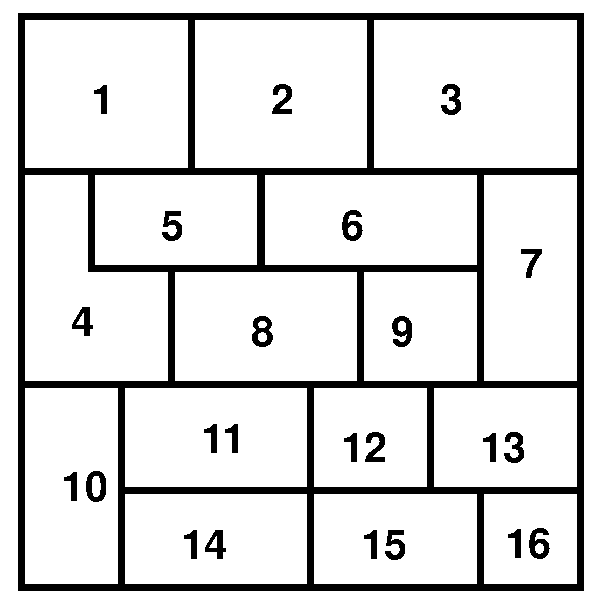
\includegraphics[width=0.5\textwidth]{SetCoveringProblemFig.pdf}
\end{center}

\begin{enumerate}
\item The city wants to build hospitals to service Annapolis. They want to make sure every district either contains a hospital, or is adjacent to another district containing a hospital. Formulate a concrete model that will allow them to make sure every district is serviced by a hospital while building the minimum number of hospitals.

{\blu

\textbf{\underline{Decision Variables}}

Let $x_1 = 1$ if a hospital is built in zone 1 and 0 otherwise \\
$\vdots$ \\
Let $x_{16} = 1$ if a hospital is build in zone 16 and 0 otherwise

\textbf{\underline{Objective Function}}

\[
\text{minimize } x_1+x_2+\cdots +x_{16}
\]

\textbf{\underline{Constraints}}

\begin{optprog*}
& x_1+x_2+x_4+x_5 & \geq & 1 & \text{(Zone 1 is covered)} \\
& x_1+x_2+x_3+x_5+x_6 & \geq & 1 & \text{(Zone 2 is covered)} \\
& \vdots \\
& x_{13}+x_{15}+x_{16} & \geq & 1 & \text{(Zone 16 is covered)} \\
& x_1, x_2, \ldots, x_{16} & \in & \{0,1\} & \text{(binary)}
\end{optprog*}


}

\item Convert your concrete model from part 1 into a parameterized model \emph{Hint: It may be helpful to define some extra sets that aren't directly in the problem or use the adjacency matrix idea from class}.

{\blu There are two ways to solve this problem. The first uses an extra parameter. The second uses extra sets. Both options should make sense to you. I'll give the first option below in green and the second option in red.}

{\color{teal} OPTION 1

\textbf{\underline{Sets}}

Let $Z$ be the set of zones

\textbf{\underline{Parameters}}

Let $a_{i,j} = 1$ if zone $i$ is adjacent to zone $j$ for all $i \in Z$ and all $j \in Z$. (Note that this is a parameter not a variable).

\textbf{\underline{Decision Variables}}

Let $x_i = 1$ if a hospital is build in zone $i$ for all $i \in Z$

\textbf{\underline{Objective Function}}

\[
\text{min } \sum_{i \in Z} x_i
\]

\textbf{\underline{Constraints}}

\begin{optprog*}
& \sum_{i \in Z} a_{i,j} x_i & \geq & 1 & \text{for all $j \in Z$} \\
& x_i & \in & \{0,1\} & \text{for all $i \in Z$}
\end{optprog*}

}


\newpage

{\color{red} OPTION 2

\textbf{\underline{Sets}}

Let $Z$ be the set of zones \\
Let $N_i$ be the set of zones that can cover node $i$ for all $i \in Z$ (thus $N_1 = \{1,2,4,5\}$, $N_2 = \{1,2,3,5,6\}$, etc)

\textbf{\underline{Parameters}}

None

\textbf{\underline{Decision Variables}}

Let $x_i = 1$ if a hospital is build in zone $i$ for all $i \in Z$

\textbf{\underline{Objective Function}}

\[
\text{min } \sum_{i \in Z} x_i
\]

\textbf{\underline{Constraints}}

\begin{optprog*}
& \sum_{j \in N_i} x_i & \geq & 1 & \text{for all $i \in Z$} \\
& x_i & \in & \{0,1\} & \text{for all $i \in Z$}
\end{optprog*}
}

\end{enumerate}












\end{document}
